\documentclass[11pt]{beamer}
\usetheme{Boadilla}
\usepackage[utf8]{inputenc}
\usepackage{amsmath}
\usepackage{amsfonts}
\usepackage{amssymb}
\usepackage{tikz}
\usetikzlibrary{arrows,decorations.markings}
\usetikzlibrary{shapes.geometric}
\usetikzlibrary{positioning}
\usepackage[absolute,verbose,overlay]{textpos}
\usepackage{stackengine}
\usepackage{scalerel}
\usepackage{tikz-uml}
\usepackage{listings}
\usepackage{forest}
\usepackage{booktabs}
\usepackage{listings}
\usepackage{fancyvrb}
\usepackage{pgfplots}


\graphicspath{{figures/}}


\newlength\triwidth
\author{Peter M\"unch}
\title{Core Level Performance Optimization of DGEMM}
%\setbeamercovered{transparent} 
%\setbeamertemplate{navigation symbols}{} 
%\logo{} 
%\institute{IN2076 - Advanced Computer Architecture} 
\date{December 15, 2017} 
%\subject{} 

\setbeamertemplate{footline}[frame number]{}

%gets rid of bottom navigation symbols
\setbeamertemplate{navigation symbols}{}
\expandafter\def\expandafter\insertshorttitle\expandafter{%
  \insertshorttitle\hfill%
  \insertframenumber\,/\,\inserttotalframenumber}

%gets rid of footer
%will override 'frame number' instruction above
%comment out to revert to previous/default definitions
%\setbeamertemplate{footline}{}

\setbeamertemplate{bibliography item}{}



\bibliographystyle{apalike}
% make bibliography entries smaller
%\renewcommand\bibfont{\scriptsize}
% If you have more than one page of references, you want to tell beamer
% to put the continuation section label from the second slide onwards
\setbeamertemplate{frametitle continuation}[from second]
% Now get rid of all the colours
\setbeamercolor*{bibliography entry title}{fg=black}
\setbeamercolor*{bibliography entry author}{fg=black}
\setbeamercolor*{bibliography entry location}{fg=black}
\setbeamercolor*{bibliography entry note}{fg=black}

\begin{document}

\begin{frame}
\titlepage
\end{frame}

%\begin{frame}
%\tableofcontents
%\end{frame}

\newcommand{\linen}[2]{ &&\qquad #1 & #2 \\}
\newcommand{\linenn}[4]{#1 & #2 &\qquad #3 & #4 \\}
\newcommand{\linel}[1]{ &&#1 \\}

\usetikzlibrary{decorations.text}
\definecolor{mygray}{RGB}{208,208,208}
\definecolor{mymagenta}{RGB}{226,0,116}
\newcommand*{\mytextstylee}{\sffamily\bfseries\color{white!85}}
\newcommand*{\mytextstyle}{\sffamily\bfseries\color{black!85}}
\newcommand{\arcarrow}[3]{%
   % inner radius, middle radius, outer radius, start angle,
   % end angle, tip protusion angle, options, text
   \pgfmathsetmacro{\rin}{2.5}
   \pgfmathsetmacro{\rmid}{3.0}
   \pgfmathsetmacro{\rout}{3.5}
   \pgfmathsetmacro{\astart}{#1}
   \pgfmathsetmacro{\aend}{#2}
   \pgfmathsetmacro{\atip}{5}
   \fill[mygray, very thick] (\astart+\atip:\rin)
                         arc (\astart+\atip:\aend:\rin)
      -- (\aend-\atip:\rmid)
      -- (\aend:\rout)   arc (\aend:\astart+\atip:\rout)
      -- (\astart:\rmid) -- cycle;
   \path[
      decoration = {
         text along path,
         text = {|\mytextstyle|#3},
         text align = {align = center},
         raise = -1.0ex
      },
      decorate
   ](\astart+\atip:\rmid) arc (\astart+\atip:\aend+\atip:\rmid);
}
\newcommand{\arcarroww}[3]{%
   % inner radius, middle radius, outer radius, start angle,
   % end angle, tip protusion angle, options, text
   \pgfmathsetmacro{\rin}{2.5}
   \pgfmathsetmacro{\rmid}{3.0}
   \pgfmathsetmacro{\rout}{3.5}
   \pgfmathsetmacro{\astart}{#1}
   \pgfmathsetmacro{\aend}{#2}
   \pgfmathsetmacro{\atip}{5}
   \fill[blue, very thick] (\astart+\atip:\rin)
                         arc (\astart+\atip:\aend:\rin)
      -- (\aend-\atip:\rmid)
      -- (\aend:\rout)   arc (\aend:\astart+\atip:\rout)
      -- (\astart:\rmid) -- cycle;
   \path[
      decoration = {
         text along path,
         text = {|\mytextstylee|#3},
         text align = {align = center},
         raise = -1.0ex
      },
      decorate
   ](\astart+\atip:\rmid) arc (\astart+\atip:\aend+\atip:\rmid);
}


\section{Introduction}

\begin{frame}[fragile]{\textcolor{blue}{Introduction}}

\textcolor{blue}{DGEMM} (double-precision matrix-matrix multiplication) as:
\begin{itemize}
\item sequence of \textcolor{blue}{$m \times n$ dot-products $\rightarrow$ jik}:

\begin{small}
\begin{figure}
   % \centering
    \def\svgwidth{0.7\columnwidth}
    \input{figures/dot.pdf_tex}
\end{figure}
\end{small}

\item sequence of \textcolor{blue}{$n$ matrix-vector-multiplication $\rightarrow$ jki}:
\begin{small}
\begin{figure}
   % \centering
    \def\svgwidth{0.7\columnwidth}
    \input{figures/tensor.pdf_tex}
\end{figure}
\end{small}

\item sequence of \textcolor{blue}{$p$ outer-products $\rightarrow$ kji}
\end{itemize}

\begin{textblock}{5}(4.7,5.4)
{\tiny (i,j)}
\end{textblock}

\end{frame}

\begin{frame}[fragile]{\textcolor{blue}{Introduction (cont.)}}

\lstset { %
    language=C++,
    backgroundcolor=\color{blue!10}, % set backgroundcolor
    basicstyle=\footnotesize,% basic font setting,
        commentstyle=\color[rgb]{0.026,0.112,0.095},
                basicstyle=\ttfamily,
                keywordstyle=\color{blue}\ttfamily,
                stringstyle=\color{red}\ttfamily,
                commentstyle=\color{gray}\ttfamily,
                morecomment=[l][\color{magenta}]{\#}
}

Baseline implementation of DGEMM :
%(double-precision matrix-matrix multiplication)
\begin{footnotesize}
\begin{lstlisting}[language=C++]
#define A( i, j ) A[(j)*lda + (i)] // column-major order
/* same for B and C */

void bl_dgemm(int m, int n, int k, double *A, int lda, 
	double *B, int ldb, double *C, int ldc) {

  for (int j = 0; j < n; j++) // perform GAXPY
      for (int k = 0; k < p; k++)
          for (int i = 0; i < m; i++)
              C( i, j ) += A( i, k ) * B( k, j );

}
\end{lstlisting}
\end{footnotesize}

\begin{itemize}
\item Library implementations: BLAS, \textcolor{blue}{BLIS},  CBLAS, Intel MKL
\item Following discussion based on \textcolor{blue}{BLISLab}\footnote{\url{https://github.com/flame/blislab} and papers related to BLIS (see later)}: step-by-step hands-on for DGEMM implementation in BLIS
\end{itemize}

\end{frame}


\begin{frame}{\textcolor{blue}{Table of Contents}}

\tableofcontents

\end{frame}

\section{Performance Optimization Process}

\begin{frame}{\textcolor{blue}{Performance Optimization Process}\footnote{adopted from Baruffa et al. 2017}}


\begin{center}
\begin{tikzpicture}
   \fill[even odd rule,white] circle (2.5);

   \node at (0,0) [
      font  = \mytextstyle,
      color = white,
      align = center
   ]{
      PDCA\\
      Cycle
   };
   \arcarrow{ 85}{  23}{Scalar opt.}
   \arcarroww{-49}{20}{Vectorization}
   \arcarroww{-121}{-47}{Memory access}
   \arcarrow{167}{241}{Multi-threading}
   \arcarrow{ 162}{95}{Communication}
\end{tikzpicture}
\end{center}

\begin{textblock}{6}(10.8,1.3)
\begin{itemize}
\item compiler flags
\item data casting
\item precision consistency
\end{itemize}
\end{textblock}


\begin{textblock}{6}(11.8,10)
\begin{itemize}
\item SIMD
%\item 
\end{itemize}
\end{textblock}

\begin{textblock}{10}(4.0,13.5)
\begin{itemize}
\item improve data layout, cache access
\end{itemize}
\end{textblock}


\begin{textblock}{6}(0,10)
\begin{itemize}
\item OpenMP
\item scheduling
\item pinning
\end{itemize}
\end{textblock}


\begin{textblock}{6}(1,2.3)
\begin{itemize}
\item MPI
\item offloading
\end{itemize}
\end{textblock}

\end{frame}

\RecustomVerbatimCommand{\VerbatimInput}{VerbatimInput}%
{fontsize=\scriptsize,
 %
 %frame=lines,  % top and bottom rule only
 framesep=2em, % separation between frame and text
 %rulecolor=\color{Gray},
 %
 %label=\fbox{\color{Black}data.txt},
 labelposition=topline,
 %
 commandchars=\|\(\), % escape character and argument delimiters for
                      % commands within the verbatim
 commentchar=\#        % comment character
}

\section{Hardware}

\begin{frame}[fragile]{\textcolor{blue}{Hardware limits}}

\begin{minipage}{0.42\textwidth}
%\scalebox{0.5}{
\VerbatimInput{code/likwid-topology.txt}
%}
\end{minipage}~
\begin{minipage}{0.49\textwidth}

\vspace{3.0cm}

\textcolor{blue}{Peak performance per core}

\quad= clock speed * Flops/instruction

\quad= 2.60GHz * 16 Flops/instruction

\quad$\approx$ \textcolor{blue}{41.6 GFlops/sec}

\vspace{0.5cm}

Peak performance can be reached  since DGEMM = \textcolor{blue}{compute-bound}


\quad $\rightarrow$ see also: \textcolor{blue}{Roofline model}\footnote{Williams et al. 2009}

\vspace{1.0cm}

\end{minipage}


\section{Implementation}

\subsection{Ingredient 1: Micro-kernel}

\end{frame}

\begin{frame}[fragile]{\textcolor{blue}{Ingredient 1: Micro-kernel}}

\textcolor{blue}{Unrolling} e.g.\footnote{for AVX2:  McCalpin 2016 
%\url{https://sites.utexas.edu/jdm4372/2016/11/05/intel-discloses-vectorsimd-instructions-for-future-processors/}
}: \textcolor{blue}{4 $\times$ i}, \textcolor{blue}{3 $\times$ j}, \textcolor{blue}{4 $\times$ k} implies a  sequence of \textcolor{blue}{rank-1 updates}:

\begin{small}
\begin{figure}
    \centering
    \def\svgwidth{0.4\columnwidth}
    \input{figures/micro1.pdf_tex}\qquad
    \def\svgwidth{0.4\columnwidth}
    \input{figures/micro3.pdf_tex}
    
    \vspace{0.2cm}
    
    \def\svgwidth{0.4\columnwidth}
    \input{figures/micro2.pdf_tex}\qquad
    \def\svgwidth{0.4\columnwidth}
    \input{figures/micro4.pdf_tex}
\end{figure}
\end{small}
%
%Implement via a limited set of \textcolor{blue}{Intel Intrinsics} commands:
%\begin{itemize}
%\item \_\_m256d + FMA
%\item \_mm256\_setzero\_pd()
%\item \_mm256\_loadu\_pd()
%\item \_mm256\_broadcast\_sd()
%\end{itemize}

Implement via a limited set of \textcolor{blue}{AVX2 Intel Intrinsics} commands:

\vspace{0.3cm}

\begin{minipage}{0.5\textwidth}
\begin{itemize}
\item \_\_m256d + FMA 
\item \_mm256\_setzero\_pd()
%\item \_mm256\_loadu\_pd()
%\item \_mm256\_broadcast\_sd()
\end{itemize}
\end{minipage}~
\begin{minipage}{0.5\textwidth}
\begin{itemize}
%\item \_\_m256d + FMA
%\item \_mm256\_setzero\_pd()
\item \_mm256\_loadu\_pd()
\item \_mm256\_broadcast\_sd()
\end{itemize}
\end{minipage}

\vspace{0.7cm}

\qquad\qquad\qquad\qquad\qquad\qquad\qquad ... or alternatively \textcolor{blue}{via Inline Assembler}

%\begin{minipage}{0.5\textwidth}
%\begin{small}
%\begin{figure}
%    \centering
%    \def\svgwidth{0.9\columnwidth}
%    \input{figures/micro1.pdf_tex}
%    
%    \vspace{0.2cm}
%    
%    \def\svgwidth{0.9\columnwidth}
%    \input{figures/micro2.pdf_tex}
%    
%    \vspace{0.2cm}
%    
%    \def\svgwidth{0.9\columnwidth}
%    \input{figures/micro3.pdf_tex}
%    
%    \vspace{0.2cm}
%    
%    \def\svgwidth{0.9\columnwidth}
%    \input{figures/micro4.pdf_tex}
%\end{figure}
%\end{small}
%\end{minipage}~
%\begin{minipage}{0.5\textwidth}
%
%\lstset { %
%    language=C++,
%    backgroundcolor=\color{blue!10}, % set backgroundcolor
%    basicstyle=\footnotesize,% basic font setting,
%        commentstyle=\color[rgb]{0.026,0.112,0.095},
%                basicstyle=\ttfamily,
%                keywordstyle=\color{blue}\ttfamily,
%                stringstyle=\color{red}\ttfamily,
%                commentstyle=\color{gray}\ttfamily,
%                morecomment=[l][\color{magenta}]{\#}
%}
%
%\begin{footnotesize}
%\begin{lstlisting}[language=C++]
%c_0.v = _mm256_setzero_pd();
%c_1.v = _mm256_setzero_pd();
%c_2.v = _mm256_setzero_pd();
%
%for (int p = 0; p < k; p += 4) {
%  a_0.v = _mm256_loadu_pd((double *) (a + 0));
%            a_1.v = _mm256_loadu_pd((double *) (a + 4));
%            a_2.v = _mm256_loadu_pd((double *) (a + 8));
%            a_3.v = _mm256_loadu_pd((double *) (a + 12));
%
%            // 0
%            b_0.v = _mm256_broadcast_sd((double *) (b + 0));
%            b_1.v = _mm256_broadcast_sd((double *) (b + 1));
%            b_2.v = _mm256_broadcast_sd((double *) (b + 2));
%
%            c_0.v += a_0.v * b_0.v;
%            c_1.v += a_0.v * b_1.v;
%            c_2.v += a_0.v * b_2.v;
%\end{lstlisting}
%\end{footnotesize}
%
%\end{minipage}


\end{frame}

\begin{frame}{\textcolor{blue}{Ingredient 1: Micro-kernel (cont.)}}

More general (micro-kernel embedded into the multiplication of matrices of arbitrary shape):

\begin{small}
\begin{figure}
    \centering
    \def\svgwidth{0.95\columnwidth}
    \input{figures/micro5.pdf_tex}
\end{figure}
\end{small}

\begin{itemize}
\item \textcolor{blue}{vectorized} and by definition: \textcolor{blue}{register blocked}
  $\rightarrow$   can we do better?
\item be aware of corner cases
\end{itemize}

\end{frame}


\subsection{Ingredient 2: Blocking}

\begin{frame}{\textcolor{blue}{Ingredient 2: Blocking}}

Basic idea: \textcolor{blue}{perform small DGEMM on tiles}

\vspace{0.5cm}

\begin{small}
\begin{figure}
    \centering
    \def\svgwidth{0.7\columnwidth}
    \input{figures/tiles.pdf_tex}
\end{figure}
\end{small}

\qquad\qquad$\rightarrow$ such that \textcolor{blue}{tiles stay in cache} during multiplication

\qquad\qquad$\rightarrow$ such that \textcolor{blue}{one tile can be reused} during next multiplication

\end{frame}


\begin{frame}{\textcolor{blue}{Ingredient 2: Blocking\footnote{adopted from Smith et al. 2014} (cont.)}}
\begin{small}
\begin{figure}
    \centering
    \def\svgwidth{0.9\columnwidth}
    \input{figures/algo.pdf_tex}
\end{figure}
\end{small}

\end{frame}

\subsection{Putting All Together}

\begin{frame}{\textcolor{blue}{Putting All Together}}

\textcolor{blue}{Data alignment}, \textcolor{blue}{arrray padding}, \textcolor{blue}{software prefetching}, and 

\qquad\qquad choosing the \textcolor{blue}{tile sizes in BLISLab}:
%\begin{align*}
%MC= 72\quad NC = 4048 \quad KC = 256 \quad MR = 8 \quad NR = 6 
%\end{align*}

\vspace{-0.2cm}

%\begin{align*}
%\textcolor{blue}{|\tilde{A}|} &\le MC \times KC \approx  144kB \textcolor{blue}{\le 256kB}\\
%\textcolor{blue}{|\tilde{B}|} &\le KC \times NC \approx  8MB \textcolor{blue}{\le 30MB}\\
%\textcolor{blue}{|sliver\,of\,\tilde{B}|} &\le KC \times NR \approx  12kB \textcolor{blue}{\le 32kB}\\
%\end{align*}

\begin{small}
\begin{figure}
    \centering
    \def\svgwidth{0.9\columnwidth}
    \input{figures/algo-mem.pdf_tex}
\end{figure}
\end{small}

\vspace{0.1cm}

Further details on \textcolor{blue}{BLIS} in:

\qquad Goto et al. 2008, Smith et al. 2014, Zee et al. 2015, Zee et al. 2016 

\end{frame}

\begin{frame}{\textcolor{blue}{Putting All Together (cont.)}}

In the tutorial, we choose following configuration (see \textcolor{blue}{\texttt{bl\_config.h}}):
\begin{align*}
MC = 72 \quad \quad NC = 4080 \quad KC = 4080\\
MR = 8 \quad NR = 6 \qquad\qquad
\end{align*}

such that
\begin{align*}
\textcolor{blue}{|\tilde{A}|} &\le MC \times KC \approx  144kB \textcolor{blue}{\le 256kB}\\
\textcolor{blue}{|\tilde{B}|} &\le KC \times NC \approx  8MB \textcolor{blue}{\le 30MB}\\
\textcolor{blue}{|sliver\,of\,\tilde{B}|} &\le KC \times NR \approx  12kB \textcolor{blue}{\le 32kB}\\
\end{align*}

\end{frame}

\subsection{Performance Tests}

\begin{frame}[fragile]{\textcolor{blue}{Tests: Introduction}}

\textcolor{blue}{Three versions} considered\footnote{'basic' based on step 0 of BLISLab, 'vectorized' based on step 3 with MC=KC=4048, 'vectorized+blocked' based on step 3}:
\begin{enumerate}
\item basic
\item micro-kernel
\item micro-kernel + blocked
\end{enumerate}

\vspace{0.5cm}

Measurements of hardware performance counters taken with \textcolor{blue}{\texttt{likwid-perfctr}}\footnote{
%Likwid 2017
\url{https://github.com/RRZE-HPC/likwid}
}:

\lstset { %
    language=C++,
    backgroundcolor=\color{blue!10}, % set backgroundcolor
    basicstyle=\footnotesize,% basic font setting,
        commentstyle=\color[rgb]{0.026,0.112,0.095},
                basicstyle=\ttfamily,
                keywordstyle=\color{blue}\ttfamily,
                stringstyle=\color{red}\ttfamily,
                commentstyle=\color{gray}\ttfamily,
                morecomment=[l][\color{magenta}]{\#}
}

\begin{footnotesize}
\begin{lstlisting}[language=C++]
	likwid-perfctr -f -C N:0 -g CACHES -m ./main
\end{lstlisting}
\end{footnotesize}

Supported Intel Haswell EP/EN/EX performance groups: 

\qquad e.g.: \texttt{BRANCH, \textcolor{blue}{CACHES}, \textcolor{blue}{CYCLE\_ACTIVITY}, ENERGY,} 

\qquad\qquad\texttt{FALSE\_SHARE, FLOPS\_AVX, MEM, UOPS }

\end{frame}

\begin{frame}{\textcolor{blue}{Tests: Time}}

\begin{center}
\begin{tikzpicture}
\begin{axis}[
legend pos=north west, grid=both,xlabel={Matrix size N}, ylabel={Time [sec]},%xmin=2,xmax=10,minor tick num=1,
ymin=0, %ymax=45, 
xmin=0,
%title= \textbf{Overall data volume}, 
width=0.9\textwidth, height=0.7\textwidth ]
\addplot[blue,mark=triangle*,line width=1pt] table [x=size, y={Runtime (RDTSC) [s]}, col sep=comma] {data/v0/CACHES/ranks-statistics/ave.csv};

\addplot[red,mark=triangle*,line width=1pt] table [x=size, y={Runtime (RDTSC) [s]}, col sep=comma] {data/v1/CACHES/ranks-statistics/ave.csv};

\addplot[orange,mark=triangle*,line width=1pt] table [x=size, y={Runtime (RDTSC) [s]}, col sep=comma] {data/v2/CACHES/ranks-statistics/ave.csv};

%\addplot[red,mark=triangle*,line width=1pt] table [x=i, y=flop, col sep=comma] {data/v1/CACHES/0.csv};

%\addplot[orange,mark=triangle*,line width=1pt] table [x=i, y=flop, col sep=comma] {data/v2/CACHES/0.csv};
\legend{v1, v2, v3}
\end{axis}
\end{tikzpicture}
\end{center}

\end{frame}

\begin{frame}{\textcolor{blue}{Tests: Time (cont.)}}

\begin{center}
\begin{tikzpicture}
\begin{axis}[ymode=log,xmode=log,log ticks with fixed point,
legend pos=north west, grid=both,xlabel={Matrix size N}, ylabel={Time [sec]},%xmin=2,xmax=10,minor tick num=1,
ymin=0.003, ymax=1000, 
xmin=0, xmax = 6500,
%title= \textbf{Overall data volume}, 
width=0.9\textwidth, height=0.7\textwidth ]
\addplot[blue,mark=triangle*,line width=1pt] table [x=size, y={Runtime (RDTSC) [s]}, col sep=comma] {data/v0/CACHES/ranks-statistics/ave.csv};

\addplot[red,mark=triangle*,line width=1pt] table [x=size, y={Runtime (RDTSC) [s]}, col sep=comma] {data/v1/CACHES/ranks-statistics/ave.csv};

\addplot[orange,mark=triangle*,line width=1pt] table [x=size, y={Runtime (RDTSC) [s]}, col sep=comma] {data/v2/CACHES/ranks-statistics/ave.csv};


\addplot +[dashed, mark=none,line width=1pt,black] coordinates {(2048, 0.001) (2048, 1000)};


\addplot [solid, mark=none,line width=1pt,black,fill=white] coordinates {(2500, 1) (6000, 13.8) (6000,1) (2500,1)};

%\addplot[red,mark=triangle*,line width=1pt] table [x=i, y=flop, col sep=comma] {data/v1/CACHES/0.csv};

%\addplot[orange,mark=triangle*,line width=1pt] table [x=i, y=flop, col sep=comma] {data/v2/CACHES/0.csv};
\legend{v1, v2, v3}
\end{axis}
\end{tikzpicture}
\end{center}


\begin{textblock}{5}(9,1.5)
50\% of L1 cache
\end{textblock}

\begin{textblock}{5}(12.7,7.4)
$\mathcal{O}(N^3)$
\end{textblock}

\end{frame}

\begin{frame}{\textcolor{blue}{Tests: Work}}

\begin{center}
\begin{tikzpicture}
\begin{axis}[grid=both,xlabel={Matrix size N}, ylabel={Work [GFlops/sec]},%xmin=2,xmax=10,minor tick num=1,
ymin=0, ymax=45, xmin=0,
%title= \textbf{Overall data volume}, 
width=0.9\textwidth, height=0.7\textwidth ]
\addplot[blue,mark=triangle*,line width=1pt] table [x=i, y=flop, col sep=comma] {data/v0/CACHES/0.csv};


\addplot[red,mark=triangle*,line width=1pt] table [x=i, y=flop, col sep=comma] {data/v1/CACHES/0.csv};

\addplot[orange,mark=triangle*,line width=1pt] table [x=i, y=flop, col sep=comma] {data/v2/CACHES/0.csv};


\addplot +[dashed, mark=none,line width=1pt,black] coordinates {(2048, 0) (2048, 45)};

\legend{v1, v2, v3}
\end{axis}
\end{tikzpicture}
\end{center}

\begin{textblock}{5}(6,1.1)
50\% of L1 cache
\end{textblock}

\end{frame}

\begin{frame}{\textcolor{blue}{Tests: Caches}}

\begin{center}
\begin{tikzpicture}
\begin{axis}[legend pos=north west,grid=both,xlabel={Matrix size N}, ylabel={Data volume [Byte/Flop]},%xmin=2,xmax=10,minor tick num=1,
ymin=0, ymax=16, xmin=0,
%title= \textbf{Overall data volume}, 
width=0.9\textwidth, height=0.7\textwidth ]
\addplot[blue,mark=triangle*,line width=1pt] table [x=Dimensions, y=L1<->L2, col sep=comma] {data/v0/CUSTOM/caches-datavolume.csv};
\addplot[dashed, blue ,mark=triangle*,line width=1pt] table [x=Dimensions, y=L2<->L3, col sep=comma] {data/v0/CUSTOM/caches-datavolume.csv};


\addplot[red,mark=triangle*,line width=1pt] table [x=Dimensions, y=L1<->L2, col sep=comma] {data/v1/CUSTOM/caches-datavolume.csv};
\addplot[dashed, red ,mark=triangle*,line width=1pt] table [x=Dimensions, y=L2<->L3, col sep=comma] {data/v1/CUSTOM/caches-datavolume.csv};



\addplot[orange,mark=triangle*,line width=1pt] table [x=Dimensions, y=L1<->L2, col sep=comma] {data/v2/CUSTOM/caches-datavolume.csv};
\addplot[dashed, orange ,mark=triangle*,line width=1pt] table [x=Dimensions, y=L2<->L3, col sep=comma] {data/v2/CUSTOM/caches-datavolume.csv};
\legend{v1: $L_1\leftrightarrow L_2$, v1: $L_2\leftrightarrow L_3$, v2: $L_1\leftrightarrow L_2$, v2: $L_2\leftrightarrow L_3$,v3: $L_1\leftrightarrow L_2$, v3: $L_2\leftrightarrow L_3$,}

\addplot +[mark=none,line width=1pt,black] coordinates {(2048, 0) (2048, 16)};

\end{axis}
\end{tikzpicture}
\end{center}


\begin{textblock}{5}(6,1.5)
50\% of L1 cache
\end{textblock}

\begin{textblock}{10}(5,0.5)
{\footnotesize \textcolor{red}{Worst case: (3*read + 1*write) / 2 Flops = 16 Byte/Flop}}
\end{textblock}

\begin{textblock}{5}(3.2,1.0)
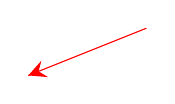
\begin{tikzpicture}
\draw [red, decoration={markings,mark=at position 1 with
    {\arrow[scale=2,>=stealth]{>}}},postaction={decorate}] (0,0) -- (-1.5,-0.6) ;
\end{tikzpicture}
\end{textblock}

\end{frame}


\begin{frame}{\textcolor{blue}{Tests: Instruction Cycles}}

\vspace{0.2cm}

\begin{center}
\begin{tikzpicture}
\begin{axis}[legend columns=4,legend pos=north west,%ybar,
 grid=both,xlabel={Matrix size N}, ylabel={Total cycles without execution [\%]}, bar width=2pt, minor tick num=1,ymin=0, ymax=65,
%title=\textbf{Cycles without execution}, 
width=0.9\textwidth, height=0.7\textwidth ]
%\addplot table [x=Dimensions, y=All, col sep=comma] {data/v1/CUSTOM/cycle-activity-without.csv};
%\addplot table [x=Dimensions, y=L1, col sep=comma] {data/v1/CUSTOM/cycle-activity-without.csv};
%\addplot table [x=Dimensions, y=L2, col sep=comma] {data/v1/CUSTOM/cycle-activity-without.csv};
\addplot [blue ,mark=square*,line width=1pt] table [ x=Dimensions, y=MEM, col sep=comma] {data/v0/CUSTOM/cycle-activity-without.csv};
\addplot [red ,mark=square*,line width=1pt] table [ x=Dimensions, y=MEM, col sep=comma] {data/v1/CUSTOM/cycle-activity-without.csv};
\addplot [orange ,mark=square*,line width=1pt] table [x=Dimensions, y=MEM, col sep=comma] {data/v2/CUSTOM/cycle-activity-without.csv};

\addplot +[dashed, mark=none,line width=1pt,black] coordinates {(2048, 0) (2048, 65)};

\legend{v1, v2, v3}
\end{axis}
\end{tikzpicture}
\end{center}


\begin{textblock}{5}(6,1.5)
50\% of L1 cache
\end{textblock}

\end{frame}


\section{Outlook}

\begin{frame}{\textcolor{blue}{Outlook}}

\begin{itemize}
\item \textcolor{blue}{Cache-oblivious algorithms} (Frigo 1999): recursive implementation with little to no knowledge of the given hardware:
\begin{align*}
\left(
\begin{array}{c}
A_1\\ A_2
\end{array}
\right) B &= 
\left(
\begin{array}{c}
A_1 B\\ A_2 B
\end{array}
\right) \\
\left(\begin{array}{cc}
A_1 & A_2
\end{array}\right) 
\left(\begin{array}{c}
B_1\\ B_2
\end{array}\right)
&= 
A_1B_1+A_2B_2 \\
A\left(\begin{array}{cc}
B_1 & B_2
\end{array}\right)
&= 
\left(\begin{array}{cc}
AB_1 & AB_2
\end{array}\right)
\end{align*}
\item Threaded and distributed implementation: \textcolor{blue}{Cannon's algorithm} (Cannon 1969) and \textcolor{blue}{SUMMA} (Geijn et al. 1999)
\item Fault tolerance: \textcolor{blue}{checksums} (Bosilca et al. 2009)
\end{itemize}

\end{frame}

\section{References}

\begin{frame}[t,allowframebreaks,plain]
\frametitle{{\color{blue}References}}
\vspace{0cm}
{\scriptsize \bibliography{literature.bib}}
\end{frame}



\end{document}